\documentclass{report}
\usepackage{xeCJK}
\setCJKmainfont{宋体}
\setCJKfamilyfont{song}{宋体}

% 宏包在这里添加.
\usepackage[colorlinks, linkcolor=red, anchorcolor=blue,
citecolor=black]{hyperref}
% 用来画图.
\usepackage{tikz}

\usepackage{amsmath}

%定理。
\usepackage{amsthm}
% 算法.
\usepackage{algorithm}
% 伪代码.
\usepackage{algpseudocode}
% 标题形式,可以去掉.
\usepackage[small,center,pagestyles]{titlesec}
\titleformat{\chapter}[hang]{\centering\Large\bfseries}{第 \thechapter 章}{1em}{}
\titlespacing{\chapter}{0pt}{*0}{*4}
\usepackage{booktabs}
% 箭头.
%\usepackage{pgflibraryarrows}
%\usepackage{pgflibrarysnakes}

\usepackage{subfig}

%%%%%%%%%%%%%%%%%%%%%%%%%%%%%%%%%%%%%%%%%%%%%%%%%%%%%%%%%%%%%%%%%
\newtheorem{theorem}{Theorem}[section]
\theoremstyle{Remark}
\newtheorem{Remark}[theorem]{Remark}

\begin{document}

\begin{abstract}
   Navier-Stokes 方程是一种简化的流体模型, 模拟自然界的流体, 从大尺度
   的海洋洋流,到小尺度的血管流。深入研究这个流体模型,有助于我们更好
   的了解自然。Navier-Stokes 方程中有非线性项,并且当流速很大的时候,
   求解会很困难,并且在三维的情况下,还会有湍流出现。因此,研究
   Navier-Stokes 方程的数值解法是有意义的。
 
   本文主要是在嵌套的两层网格,结合移动网格方法,用低阶混合元方法来
   求解Navier-Stokes方程,

\end{abstract}   

\chapter{引言}
     众所周知, 混合元是求解不可压Navier-Stokes方程的一种重要方法。为了
     保证解的唯一性,需要使速度和压力两个解的空间满足LBB条件。其中一种
     办法是使得速度空间相对压力空间来说,自由度足够多,例如Taylor-Hood
     元。另外一中方法是对压力空间施加一些约束,比如说稳定化的P1P1元,
     P1P0元。为了减少计算量,提高计算效率,通常会运用自适应网格方法。
     在文献\cite{danaila2014newton},\cite{ebeida2009unsteady}
     \cite{berrone2009space}中,运用了h-自适应的P2P1元。在实际的工程计
     算中,我们通常倾向于使用线性元,而非高次元。
     \cite{zheng2010posteriori}提出自适应网格和稳定化P1P1元、P1P0元相
     结合. \cite{di2005moving}将移动网格方法应用到不可压Navier-Stokes
     方程的求解。我们移动网格部分的策略是基于文献\cite{di2005moving}中
     的工作。然而,不稳定的有限元对应用到h-自适应上有一定的技术困难。
     综合以上考虑,我们选取稳定的P1ISOP2P1元,它自然满足LBB条件,详细见
     \cite{bercovier1979error}. 在P1ISOP2P1元,速度单元所在的网格可以有压
     力单元的网格加密一次得到,如Figure (\ref{fig::p-v})注意到在速度单元
     $u$ 和压力单元$p$ 上均是线性元。但是,速度单元网格上的6个基函数不
     在同一个速度单元上。因此在拼装散度块矩阵,即拼装压力单元和速度
     单元,这个过程并不显然。

     在本文的工作中,我们选取4P1-P1元,它与ISOP2P1拥有相同的网格结构,
     自然也满足inf-sup条件,但需要指出的是速度单元上的基函数都局部的位
     于相同的速度单元上。这给我们拼装散度块矩阵提供了便利:只要我们建
     立四个速度单元和大的压力单元之间的索引。索引的建立又依赖于两层网
     格的数据结构,这种网格结构与\cite{li2005multi}中提出的几何遗传树
     是一致的。

     基于这种网格遗传树的结构,我们可以很容易的建立四个小的速度单元与
     压力宏单元间的索引。同时在\cite{li2005multi}中h-自适应方法也是基
     于这种树结构。自然的,我们可以将h-自适应方法应用到4P1-P1元上。自
     适应网格可以减少计算量,同时可以研究流体局部小尺度上的现象,比如
     涡。同时,移动网格网格方法也可以应用在4P1-P1元上,网格移动我们只
     移动压力网格,当压力网格移动完,速度网格由压力网格加密一次即可得
     到。但是需要注意的是,求解不可压的Navier-Stokes方程,在将旧网格的
     解插值到移动后的网格的过程,要满足散度为0的条件,这个工作由
     \cite{di2005moving}中给出。

     本文的框架组织如下:在第二章中,我们介绍Navier-Stokes方程的知识。
     在第三章中我们展示4P1-P1的数据结构,接下来我们用4P1-P1元近似
     Navier-Stokes方程。移动网格的策略将在第五章中给出。最后,我们给出
     数值例子。

    \begin{figure}
      \centering    
      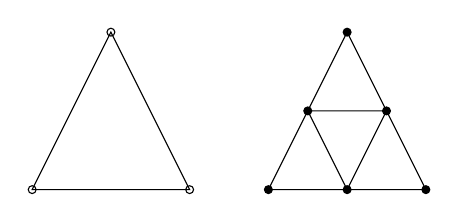
\begin{tikzpicture}
        % 三角形
        \draw (2, 1) -- (4, 1) -- (3, 3) -- cycle;
        % 三个顶点
        \draw (2, 1) circle(0.05cm);
        \draw (4, 1) circle(0.05cm);
        \draw (3, 3) circle(0.05cm);
        % 四个三角形
        \draw (5, 1) -- (6, 3) -- (7, 1) -- cycle;
        \draw (5.5, 2) -- (6.5, 2) -- (6, 1) -- cycle;
        % 六个顶点
        \draw [fill = black] (5, 1) circle(0.05cm);
        \draw [fill = black] (6, 3) circle(0.05cm);
        \draw [fill = black] (7, 1) circle(0.05cm);
        \draw [fill = black] (5.5, 2) circle(0.05cm);
        \draw [fill = black] (6.5, 2) circle(0.05cm);
        \draw [fill = black] (6, 1) circle(0.05cm);
      \end{tikzpicture}
      \caption{左: 压力 $p$ 单元, $\circ$ 为$p$单元上的自由度; 
               右: 4个速度$v$ 单元, $\bullet$ 表示$v$单元上的自由度.}
      \label{fig::p-v}       
    \end{figure}

\chapter{流体方程}
    无量纲化的不可压Navier-Stokes方程如下:
    \begin{equation}
      \begin{array}{rcl}
        \frac{\partial \vec{u}}{\partial t}-\nu \nabla^2 \vec{u} +
        \vec{u} \cdot \nabla \vec{u} + \nabla p & =
        & \vec{f},\\
        \nabla \cdot \vec{u} & = & 0,
      \end{array}
      \label{eq::NS}
    \end{equation}
    其中$\nu$为粘性系数,求解区域为$\Omega$。系统(\ref{eq::NS})的初边
    值问题如下:
    \begin{equation}
      \begin{array}{ll}
        \vec{u} = \vec{w},& \mbox{ on } \partial \Omega_D \times [0,
        T]\\
        \nu \displaystyle \frac{\partial \vec{u}}{\partial n} - p =
        \vec{0}, & \mbox{ on } \partial \Omega_N \times [0, T],  \\
        \vec{u}|_{t = 0} = \vec{u_0}, & \mbox{ in } \Omega. 
      \end{array}
      \label{eq::bc}
    \end{equation} 
    其中边界$\partial \Omega = \partial \Omega_D \bigcup \partial \Omega_N$,
    $\vec{n}$表示边界的外法向。令$L$表示区域$\Omega$的特征长度,$U$是
    入流边界上的最大流速,那么雷诺数定义为:
    \begin{equation}
      Re := \frac{UL}{\nu}.
    \end{equation}


\chapter{数据结构}

   4P1-P1是基于两套不同的网格和两种有限元空间。速度网格可以由压力网格
   全局加密一次得到。网格的数据结构是基于\cite{li2005multi}中的几何遗
   传树结构,如Figure(\ref{fig::hgrometrytree})所示。一个宏压力单元对
   应这四个速度单元,通过遍历一次所有的速度单元,利用几何遗传树结构,
   就可以建立速度单元和压力单元的$1-1$对应,如
   algorithmic(\ref{alg::index})。索引建立后,我们用P1元来拼
   装散度矩阵。

   \begin{figure}[h]
     \subfloat[全局加密一次的网格]{
       \begin{minipage}[t]{0.4\textwidth}
         \centering
         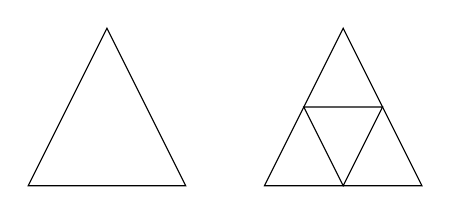
\begin{tikzpicture}
           % 三角形
           \draw (2, 1) -- (4, 1) -- (3, 3) -- cycle;
           \draw (5, 1) -- (6, 3) -- (7, 1) -- cycle;
           \draw (5.5, 2) -- (6.5, 2) -- (6, 1) -- cycle;
         \end{tikzpicture}
       \end{minipage}
     }
     \subfloat[它的几何遗传树]{
       \begin{minipage}[t]{0.6\textwidth}
         \centering
         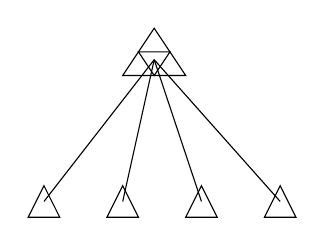
\begin{tikzpicture}
           %五个小三角形
           \draw (1.0, 0.0) -- (1.2, 0.4) -- (1.4, 0.0) -- cycle;
           \draw (2.0, 0.0) -- (2.2, 0.4) -- (2.4, 0.0) -- cycle;
           \draw (3.0, 0.0) -- (3.2, 0.4) -- (3.4, 0.0) -- cycle;
           \draw (4.0, 0.0) -- (4.2, 0.4) -- (4.4, 0.0) -- cycle;
           \draw (2.6, 2.4) -- (2.2, 1.8) -- (3.0, 1.8) -- cycle;
           \draw (2.4, 2.1) -- (2.6, 1.8) -- (2.8, 2.1) -- cycle;
           %四条线
           \draw (2.6, 2.0) -- (1.2, 0.2);
           \draw (2.6, 2.0) -- (2.2, 0.2);
           \draw (2.6, 2.0) -- (3.2, 0.2);
           \draw (2.6, 2.0) -- (4.2, 0.2);
         \end{tikzpicture}
       \end{minipage}
     }
     \caption{几何遗传树结构}
     \label{fig::hgrometrytree}
   \end{figure}

   \begin{algorithm}
     \caption{构建速度单元和压力单元间的索引}
     \begin{algorithmic}[1]
       \State \text{achieveiterator} $\gets$ \text{irregualerMeshV.beginActiveElement()}
       \State \text{enditerator} $\gets$ \text{irregualerMeshV.endActiveElement()}
     
       \While {\text{achieveiterator} $\neq$ \text{enditerator}}
           \State \text{int index-v-element} $\gets$
                   \text{achieveiterator}$-\rangle$ \text{index}
           \State \text{HElement} $\langle$ \text{DIM,
                   DIM}$\rangle \ast$ \text{parent} $\gets$
                   \text{activeiterator}$-\rangle$ \text{parent}
           \State \text{int index-p-element} $\gets$
                   \text {parent}$-\rangle$ \text{index}
           \State \text{int n-child} $\gets$
                   \text{parent}$-\rangle$ \text{n-child}
           \State
                  \text{index-p2v[index-p-element].resize}(\text{n-child})
           \While {$i \geq 0$ \textbf{and} $i < \text{n-child}$}
                  \State \text{HElement}$\langle$\text{DIM,DIM}$\rangle$ $\ast$\text{chi}
                         $\gets$ \text{parent}$-\rangle$\text{child[i]}
                  \State \text{int index-v-element} $\gets$
                         \text{child}$-\rangle$\text{index}
                  \State \text{index-p2v[index-p-element][i]} $\gets$
                         \text{index-v-element}
                  \State \text{index-v2p[index-v-element]} $\gets$ \text{index-p-element}       
           \EndWhile
       \EndWhile
     \end{algorithmic}
     \label{alg::index}
   \end{algorithm}

\chapter{有限元近似}

   我们定义解和检验空间如下:
   \begin{eqnarray}
     \mathbf{H}_E^1 & := & \left\{ \vec{u} \in \mathcal{H}^1(\Omega)^d \big|
       \vec{u} = \vec{w} \mbox{ on } \partial \Omega_D \right\},\\
     \mathbf{H}_{E_0}^1 & := & \left\{ \vec{v} \in \mathcal{H}^1(\Omega)^d \big|
       \vec{u} = \vec{0} \mbox{ on } \partial \Omega_D \right\},
   \end{eqnarray}
   那么变分形式为:寻找$(\vec{u}, p) \in (\mathbf{H}_E^1,
   L_2(\Omega))$ 使得
   \begin{eqnarray}
     \int_{\Omega}\frac{\partial \vec{u}}{\partial t} \cdot \vec{v} + 
     \nu \int_\Omega \nabla \vec{u} : \nabla \vec{v} + \int_\Omega \left(
       \vec{u} \cdot \nabla \vec{u} \right) \cdot \vec{v} - \int p
     \left( \nabla \cdot \vec{v} \right) & = & \int_\Omega \vec{f} \cdot
     \vec{v}, \label{eq::generalweak_momentum}\\
     & & \forall \vec{v} \in \mathbf{H}_{E_0}^1,\notag \\
     \int_\Omega q \left( \nabla \cdot \vec{u} \right) & = & 0,
     \label{eq::generalweak_mass} \\
     & & \forall q \in L_2(\Omega). \notag
   \end{eqnarray}

   其中$\nabla \vec{u} : \nabla \vec{v}$ 表示纯量的乘积,在二维中为
   $\nabla u_x \cdot \nabla v_x + \nabla u_y \cdot \nabla v_y$.

   假设$\tau_h$是$\Omega$ 上对压力网格的三角剖分,网格尺度 $h = max_{T
     \in \tau_h} diam(T)$, $T$ 为三角剖分 $\tau_h$ 的单元。对应的,
   $\tau_{\frac{h}{2}}$ 是对速度网格的三角剖分。基于
   $\tau_{\frac{h}{2}}$ 和 $\tau_{h}$ 上的有限元空间 $X_E^h$ 和 $P_h$
   满足 
   \begin{equation}
     X_E^h \subset \mathcal{H}_E, \quad P_h \subset L_2(\Omega) 
     \notag 
   \end{equation}
  
   那么(\ref{eq::generalweak_momentum}) 和 (\ref{eq::generalweak_mass})
   可以写成如下形式: 寻找 $(\vec{u}_h, p_h) \in X_E^h \times P_h$ 使得
   \begin{equation}
     \begin{aligned}
       &\int_{\Omega}\frac{\partial \vec{u}_h}{\partial t} \cdot \vec{v}_h
       + \nu \int_\Omega \nabla \vec{u}_h : \nabla \vec{v}_h  \\
       + & \int_\Omega \left( \vec{u}_h \cdot \nabla \vec{u}_h \right)
       \cdot \vec{v}_h - \int_\Omega p_h \left( \nabla \cdot \vec{v}_h
       \right) & = &\int_\Omega \vec{f} \cdot \vec{v}_h, &\quad
       \forall \vec{v}_h \in \mathbf{X}_0^h;  \\
       & \int_\Omega q_h \left( \nabla \cdot \vec{u}_h \right) & = &0,&
       \quad \forall q_h \in P^h.
       \label{eq::discreted_weak}
     \end{aligned}
   \end{equation}

   时间方向至少三阶Runge-Kutta方法才能保证数值稳定性。
   为了简便,我们这里只用显示Euler格式:
   $\forall (\vec{v}_h, q_h) \in \mathbf{X}_0^h \times P^h$
   \begin{equation}
     \begin{aligned}
       \int_{\Omega} \frac{\vec{u}_h^{(n + 1)} -
         \vec{u}_h^{(n)}}{\delta t} + \nu \int_{\Omega} \nabla
       \vec{u}_h^{(n + 1)} : \nabla \vec{v}_h - \int_{\Omega} p_h^{(n
         + 1)} \left( \nabla \cdot \vec{v}_h \right)
       & = \int_{\Omega} \left( \vec{u}_h^{(n)} \cdot \nabla \vec{u}_h^{(n)}
       \right) &\\
       \int_{\Omega} q_h \nabla \cdot \vec{u}_h^{(n + 1)} & = 0.&
     \end{aligned}
     \label{eq::time_discreted_weak}
   \end{equation}
   令 $\{\phi_j \}_{j = 1}^n$ 和 $\{\psi_k\}_{k = 1}^m$ 分别为速度和压
   力的线性元基函数。则数值解$\vec{u}_h^{(n + 1)} = (u_{xh}^{(n + 1)},
   u_{yh}^{(n + 1)}), p_h$ 可以写成如下形式:
   \begin{equation}
     u_{xh}^{(n + 1)} = \sum_{j = 1}^n u_j \phi_j, \quad u_{yh}^{(n +
       1)} = \sum_{j = 1}^n v_j \phi_j, \quad p_h^{(n + 1)} = \sum_{k
       = 1}^m p_k \psi_k \notag
   \end{equation}
   将$u_{xh}^{(n + 1)}, u_{yh}^{(n + 1)}, p_h^{(n + 1)}$带入离散弱形式
   (\ref{eq::time_discreted_weak}) 中,可以
   得到线性方程组
   \begin{equation}
     \left[
       \begin{array}{lll}
         \frac{1}{dt} M + \nu A & 0 & B_x^T \\
         0 & \frac{1}{dt} M +\nu A  & B_y^T \\
         B_x & B_y & 0
       \end{array}
     \right]
     \left[
       \begin{array}{c}
         u_x \\
         u_y \\
         p
       \end{array}
     \right] = 
     \left[
       \begin{array}{c}
         f_x \\
         f_y \\
         g
       \end{array}
     \right],
     \label{eq::linear_system}
   \end{equation}
   其中M 是 $n \times n$ 的质量矩阵,A是拉普拉斯矩阵,由以下形式:
   \begin{eqnarray}
     A & = & [a_{ij}], \quad a_{ij} = \int_\Omega \nabla \phi_i \cdot \nabla
     \phi_j  \notag \\
     M & = & [m_{ij}], \quad m_{ij} = \int_{\Omega}\phi_i \phi_j \notag \\
     B_x^T & = & [bx^T_{ik}], \quad bx^T_{ik} = \int_{\Omega} \psi_k
     \frac{\partial{\phi_i}}{\partial x}  \notag \\
     B_y^T & = & [by^T_{ik}], \quad by^T_{ik} = \int_{\Omega} \psi_k
     \frac{\partial {\phi_i}}{\partial y}  \notag \\
     f_x & = & [f_i], \quad f_i = \int_\Omega (\frac{u_{xh}^{(n)}}{dt} - (u_{xh}^{(n)}
     \frac{\partial u_{xh}^{(n)}}{\partial x} + u_{yh}^{(n)} \frac{\partial
       u_{xh}^{(n)}}{\partial y}) \phi_i \notag \\
     f_y & = & [f_i], \quad f_i = \int_\Omega (\frac{u_{yh}^{(n)}}{dt} - (u_{xh}^{(n)}
     \frac{\partial u_{yh}^{(n)}}{\partial x} + u_{yh}^{(n)} \frac{\partial
       u_{yh}^{(n)}}{\partial y}) \phi_i \notag \\
     g & = &  [g_k],\quad  g_i = 0. \notag
   \end{eqnarray}
   
   接下来我们着重解释一下散度块矩阵$B_x B_y, B_x^T, B_y^T$的拼装。 以
   $B_x^T$为例, 令$\triangle_{v_i}$ 为一个速度单元,我们可以通过上一节建立的
   单元索引来找到对应的压力单元 $\triangle_{p_k}$(如 Figure
   (\ref{fig::matrix_assemble})). $\phi_{i_1}, \phi_{i_2}, \phi_{i_3}$
   是定义在速度单元 $\triangle_{v_i}$ 上的线性元基函数,下标 $i_1,
   i_2, i_3$ 表示该顶点上的自由度在速度全部自由度的全局编号。同时
   $\psi_{k_1}, \psi_{k_2}, \psi_{k_3}$ 是定义在压力单元
   $\triangle_{p_k}$ 上的线性元基函数,$k_1, k_2, k_3$ 代表单元
   $\triangle_{p_k}$ 上的自由度在压力全部自由度中的全局编号。 
   因此 单元 $\triangle_{p_k}$ 和 $\triangle_{v_i}$ 对 $B_x^T$ 的贡献
   为
   \begin{equation}
     \left[
     \begin{array}{lll}
       \int_{\triangle_{v_i}}\psi_{k_1} \frac{\partial
         \phi_{i_1}}{\partial x} & \int_{\triangle_{v_i}} \psi_{k_2}
       \frac{\partial \phi_{i_1}}{\partial x} & \int_{\triangle_{v_i}}
       \psi_{k_3} \frac{\partial \phi_{i_1}}{\partial x} \\
       \int_{\triangle_{v_i}} \psi_{k_1} \frac{\partial
         \phi_{i_2}}{\partial x} & \int_{\triangle_{v_i}} \psi_{k_2}
       \frac{\partial \phi_{i_2}}{\partial x} & \int_{\triangle_{v_i}}
       \psi_{k_3} \frac{\partial \phi_{i_2}}{\partial x} \\
       \int_{\triangle_{v_i}} \psi_{k_1} \frac{\partial
         \phi_{i_3}}{\partial x} & \int_{\triangle_{v_i}} \psi_{k_2}
       \frac{\partial \phi_{i_3}}{\partial x} & \int_{\triangle_{v_i}}
       \psi_{k_3} \frac{\partial \phi_{i_3}}{\partial x}
     \end{array}
   \right]
   \label{eq::element_matrix}
   \end{equation}

   将贡献矩阵 (\ref{eq::element_matrix}) 加到 $B_x^T$ 中的相应位置
   $(i_1,k_1)$, $(i_1, k_2)$, $(i_1, k_3)$, $(i_2, k_1)$, $(i_2, k_2)$,
   $(i_2,k_3)$, $(i_3, k_1)$, $(i_3, k_2)$, $(i_3, k_3)$ to  $B_x^T$. 
   上。通过遍历所有的速度单元,重复上面的操作,$B_x^T$ 拼装完成。
   $B_y^T$ 也可以同样拼装。
  
   $B_x$ 和 $B_y$ 的拼装是遍历所有的压力单元,通过单元索引,找到对应的
   四个速度单元,然后分别用压力单元和四个速度单元进行拼装。过程相似,
   便不再赘述。
   \begin{figure}
     \centering    
     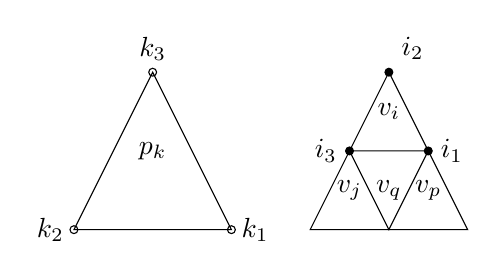
\begin{tikzpicture}
       % 三角形
       \draw (2, 1) -- (4, 1) -- (3, 3) -- cycle;
       % 三个顶点
       \draw (2, 1) circle(0.05cm);
       \draw (4, 1) circle(0.05cm);
       \draw (3, 3) circle(0.05cm);
       \draw (3, 2) node{$p_k$};
       % 三个顶点标号.
       \draw (1.7, 1) node {$k_2$};
       \draw (4.3, 1) node {$k_1$};
       \draw (3, 3.3) node {$k_3$};
       % 四个三角形
       \draw (5, 1) -- (6, 3) -- (7, 1) -- cycle;
       \draw (5.5, 2) -- (6.5, 2) -- (6, 1) -- cycle;
       % 六个顶点
       \draw [fill = black](6.5, 2) circle(0.05cm);
       \draw [fill = black](5.5, 2) circle(0.05cm);
       \draw [fill = black](6, 3) circle(0.05cm);
       % 三个顶点标号.
       \draw (6.8, 2) node {$i_1$};
       \draw (6.3, 3.3) node {$i_2$};
       \draw (5.2, 2) node {$i_3$};
       % 单元标记.
       \draw (6, 2.5) node {$v_i$};
       \draw (5.5, 1.5) node {$v_j$};
       \draw (6.5, 1.5) node {$v_p$};
       \draw (6, 1.5) node {$v_q$};
     \end{tikzpicture}
     \caption{左: $p$ 单元; 右: 与压力单元对应的4个速度$v$单元 }
     \label{fig::matrix_assemble}       
   \end{figure}

   我们主要的想法是有两套网格,速度网格和压力网格,速度网格可以由压力
   网格加密一次得到。因此我们对压力网格进行移动,然后对移动完的压力网
   格全局加密一次,即可实现对速度网格的移动。
   为了更好的说明我们的数值方法,我们将算法的流程图如Algorithm(\ref{alg::solve})所示.
   \begin{algorithm}
     \caption{移动网格方法来求解Navier Stokes方程}
     \begin{algorithmic}[1]
       \While {$t_n < T$}        
             \State 在速度网格$\triangle_v^{(n)}$和压力网格
                    $\triangle_p^{(n)}$上,求解$t = t_n$时刻
                    的 Navier-Stokes方程(\ref{eq::linear_system}), 获
                    得数值解$\vec{u}_h^{(n)}, p_h^{(n)}$. 
             \State 在压力网格$\triangle_p^{(n)}$上,用$\vec{u}_h^{(n)},
                    p_h^{(n)}$来计算控制函数, 并通过求解
                    (\ref{eq::logical}), 获得$\vec{\xi}^*$. \label{state::monitor}
             \State 判断$\parallel \vec{\xi}^* -
                    \vec{\xi}^{(0)} \parallel_{L^2}$ 是否小于容忍量
                    $\epsilon$, 如果是迭代结束,否则,继续做
                    \ref{state::start} - \ref{state::end}.
             \State 用$\vec{\xi}^* - \vec{\xi}^{(0)}$两者之差来计算
                    网格$\triangle_p^{(n)}$的移动量$\delta \vec{x}$.
                    \label{state::start}
             \State 利用\ref{state::start}中$\delta \vec{x}$, 在速度网格
                    $\triangle_v^{(n)}$上求解更新数值解的方程
                    (\ref{eq::continous_update}), 得到新网格上的中间量
                    $\vec{u}_{h, *}^{(n)}, p_{h, *}^{(n)}$.
             \State 更新$\triangle_p^{(n)}$, 通过几何遗传树结构,来
                    同步$\triangle_v^{(n)}$, 得到新的$\triangle_p^{(n
                    + 1)}$和$\triangle_v^{(n + 1)}$
             \State 回到\ref{state::monitor}. \label{state::end}
             \State 在$\triangle_v^{(n + 1)}$和$\triangle_p^{(n + 1)}$
                    上求解Navier-Stokes方程
                    (\ref{eq::linear_system}).从而真正获得$t = t_{n +
                      1}$时刻的数值解$\vec{u}_h^{(n + 1)}, p_h^{(n +
                      1)}$.
             
             \State $n = n + 1$
        \EndWhile     
     \end{algorithmic}
     \label{alg::solve}
   \end{algorithm}
\chapter{移动网格策略}

   在 $t = t_{n + 1}$ 时刻, 用上一章的方法可以得到有限元解
   $(\vec{u}_h^{(n + 1)}, p_h^{(n + 1)})$. 下面的问题是如何用新的数值
   解和旧的网格$\mathcal {T}_h^{(n)}$ 来获得新的网格$\mathcal {T}_h^{(n +
   1)}$. 我们采取文献 \cite{di2005moving} 中的方法,注意到我们区域的边
   界均是Dirichlet边界,分为以下四步:
   \section{Step 1 获取Monitor}
     选择一个合适的控制函数,对于移动网格的结果是非常重要的。应用在不
     可压Navier-Stokes方程上的控制函数主要有如下几种.
     令 $m = \frac{1}{G}$ 其中$m$是(\ref{eq::logical})中的一个纯量函数。
     关于$G$有集中不同的选择.一种是基于涡量
     \begin{equation}
       G_0 = \sqrt{1 + \alpha |\omega|^\beta}
       \label{eq::monitor_vorticity}
     \end{equation}
     其中$\omega = \nabla \times \vec{u}$, $\alpha$和$\beta$是两个正的
     常数。
     
      另外一个选择,$G$是基于数值解的梯度
      \begin{equation}
        G_1 = \sqrt{1 + \alpha |\nabla \vec{u}|^\beta}
        \label{eq::monitor_gradient}
      \end{equation}
      
      对于线性元$v_h$逼近真实解$v$,下面的后验误差估计公式可以用来近似
      计算误差
      \begin{equation}
        |v - v_h|_{1, \Omega} \sim \eta(v_h) := \sqrt{\sum\limits_{l:
            \text{内部边界}} \int_l \left[ \nabla v_h \cdot \vec{n}_l
            \right]^2 dl}
      \end{equation}
      其中$[\cdot]_l$意味着边$l$上的跳跃,即$[v]_l = v|_{l^{+}} -
      v|_{l^{+}}$. 很自然的在每个单元上等分布数值误差$\eta(v_h)$, 控制
      函数为一下形式
      \begin{equation}
        G_2 = \sqrt{1 + \alpha \eta^2(v_h)}
        \label{eq::monitor_posterror}
      \end{equation}
      \cite{di2005moving}中对(\ref{eq::monitor_posterror})进行了改进
      \begin{equation}
        G_3 = \sqrt{1 + \alpha \left[ \eta(v_h) / \text{max}\eta(v_h)
          \right]^\beta}
        \label{eq::monitor_posterror_modified}
      \end{equation}
      其中$\beta > 2$时有更好的效果。

   \section{Step 2 获取新的逻辑网格}
     求解椭圆形方程
     \begin{eqnarray}
       \begin{aligned}
         \nabla_{\vec{x}} \left ( m \nabla_{\vec{x}} \vec{\xi} \right)
         = 0 \\
         \vec{\xi} = \vec{\xi}_b 
       \end{aligned}
       \label{eq::logical}
     \end{eqnarray}
     其中 $m$ 是上一节中的纯量函数,通常依赖于$(\vec{u}_h^{(n + 1)},
     p_h^{(n + 1)})$。我们定义初始的逻辑网格$\mathcal{T}_c (\mathcal
     {A}^{0} \text{为它的节点})$。一旦初始的逻辑网格给定,在整个的求解
     过程中,将一直保持不变。通过求解(\ref{eq::logical}) 我们可以得到
     新的逻辑网格$\mathcal{T}_c^*$($\mathcal{A}^*$为它的节点)。
  \section{Step 3 物理网格的移动方向}
    
     我们先引入一些定义。$\mathcal{T}_h$ 为物理区域上的三角剖分。第i个
     点定义为$X_i$,以$X_i$ 为顶点的单元的集合称之为$T_i$。相应的计算
     区域上的标记为 $\mathcal{T}_c, \mathcal{A}_i$ 和 $T_{i,c}$。
     $\mathcal{A}_i$ 点在计算区域上的坐标定义为 $(\mathcal{A}_i^1,
     \mathcal{A}_i^2)^T$。在 Step 1 结束后,我们得到了新的逻辑网格
     $\mathcal{T}_c^*$ 和它的顶点 $\mathcal{A}_i^*$. 从而我们得到新旧
     逻辑网格的差:
     \begin{equation}
       \delta \mathcal{A}_i  = \mathcal{A}^{(0)} - \mathcal{A}_i^*
     \end{equation}
     对于一个给定的单元$E \in \mathcal{T}_h$, $X_{E_k}, 0 \leq k \leq
     2 $, 作为它的三个顶点。从$V_{\mathcal{T}_c^*}(\Omega)$ 到
     $V_{\mathcal{T}}(\Omega)$ 的分片线性映射在单元 $E$ 上的梯度是常数,
     并且满足下面的方程组:
     \begin{eqnarray}
       \begin{aligned}
        & \left (
           \begin{array}{cc}
             \mathcal{A}_{E_1}^{*, 1} - \mathcal{A}_{E_0}^{*, 1} & 
             \mathcal{A}_{E_2}^{*, 1} - \mathcal{A}_{E_0}^{*, 1} \\
             \mathcal{A}_{E_1}^{*, 2} - \mathcal{A}_{E_0}^{*, 2} &
             \mathcal{A}_{E_2}^{*, 2} - \mathcal{A}_{E_0}^{*, 2} 
           \end{array} 
         \right )
         \left (
           \begin{array}{cc}
             \frac{\partial x^1}{\partial \xi^1} & \frac{\partial
               x^1}{\partial \xi^2} \\
             \frac{\partial x^2}{\partial
               \xi^1} & \frac{\partial x^2}{\partial \xi^2}
           \end{array}
         \right ) \notag \\ = & 
         \left (
           \begin{array}{ll}
             X_{E_1}^1 - X_{E_0}^1 & X_{E_2}^1 - X_{E_0}^1 \\
             X_{E_1}^2 - X_{E_0}^2 & X_{E_2}^2 - X_{E_0}^2 
           \end{array}
         \right )
       \end{aligned}
     \end{eqnarray}

  求解上面的方程组,可以获得单元 $E$ 上的$\partial \vec{x} / \partial
  \xi$. 如果以单元的面积作为权重,则第i个点的加权平均的位移定义如下:
  \begin{eqnarray}
    \delta X_i = \frac{\sum\limits_{E \in T_i} |E| \frac{\partial
        \vec{x}}{\partial \xi}|_{\text{in} E} \delta
      \mathcal{A}_i}{\sum\limits_{E \in T_i} |E|}.
  \end{eqnarray}
  其中$|E|$代表单元$E$的面积. 为了避免网格发生缠结,在网格移动向量前乘
  上一个常量$\mu$, 即物理区域上新网格$\mathcal{T}^*$的节点表示为:
  \begin{equation}
    X_i^* = X_i + \mu \delta X_i.
  \end{equation}
  文献\cite{di2005moving}中提出$\mu$按以下方式给出:
  \begin{equation}
    \left | 
      \begin{array}{ccc}
        1 & 1 & 1 \\
        x_0^1 + \mu \delta x_0^1 & x_1^1 + \mu \delta x_1^1 & x_2^1 +
        \mu \delta x_2^1 \\
        x_0^2 + \mu \delta x_0^2 & x_1^2 + \mu \delta x_1^2 & x_2^2 +
        \mu \delta x_2 ^2 
      \end{array}
    \right | = 0
    \label{eq::muValue}
  \end{equation}
  其中$ \vec{x}_i = (x_i^1, x_i^2), 0 \leq i \leq 2$表示第i个点的坐标。
  令$\mu_i^*$ 为方程(\ref{eq::muValue})的最小正根,则令
  \begin{equation}
    \mu = \text{min} (1, \frac{\mu_i^*}{2}).
  \end{equation}
 
  \section{Step 4 散度为0的插值}
    用移动网格方法求解不可压流体时,要保证插值的过程散度是为0的。通过
    求解一个对流方程,对流的速度是网格的移动速度,从而实现旧的物理网格
    上的数值解到新的物理网格上数值解的插值。令$u_h = \sum u_i \phi_i,
    u_h \in \mathcal{X}_E^h$, $\phi_i$是有限元空间$\mathcal{X}_h$的
    基函数。引入一个虚拟的时间$\tau$, 假设基函数$\phi_i$和$u_i$均是关
    于$\tau$的函数,即$\phi_i = \phi_i(\tau), u_i = u_i(\tau)$.
    我们引入一个从旧网格$x^{\text{旧}}$到新网格$x^{\text{新}}$网格点的
    连续变换:
    \begin{equation}
       x_i(\tau) = X_i + \tau (X_i^* - X_i), \qquad \tau \in [0, 1]
       \label{eq::mesh_old2new}
    \end{equation}
    其中$X_i^* = x_i^{\text{新}}, X_i = x_i^{\text{旧}}$
    基于(\ref{eq::mesh_old2new})的连续形式$x(\tau) = x_{\text{旧}} +
    \tau (x^{\text{新}} - x^{\text{旧}})$,基函数可以定义为
    $\phi_i(\tau) = \phi_i(x(\tau))$ 并且 $u_i = u_i(x(\tau))$.
    
    在插值的过程中,我们要保持解曲线$u_h = \sum u_i \phi_i$关于$\tau$
    在弱形式下是不变的.即对$\forall \psi \in \mathcal{X}_h$,
    $(\partial_{\tau} u_h, \psi) = 0$。通过直接计算可得 
    \begin{equation}
      \frac{\partial \phi}{\partial \tau} = -\nabla_{\vec{x}} \phi_i
      \cdot \delta \vec{x}
    \end{equation}
    其中$\delta \vec{x} = x^{\text{旧}} - x^{\text{新}}$。紧接着
    \begin{eqnarray}
      \begin{aligned}
        0 & = (\partial_{\tau} u_h , \psi) \\
        & = (\partial_{\tau} \sum u_i(x(\tau)) \phi_i, \psi) \\ 
        & = (\sum \phi_i \partial u_i(x(\tau)) + \sum u_i \partial_{\tau}
        \phi_i) \\ 
        & =  (\sum \phi_i \partial_{\tau} u_i(x(\tau)) -\sum u_i
        \nabla_{\vec{x}}\phi_i \cdot \delta \vec{x}, \psi) \\
        & =  (\sum \phi_i \partial_{\tau} u_i(x(\tau)) - \nabla_{\vec{x}}u_h
        \cdot \delta \vec{x}, \psi)
     \end{aligned}
     \label{eq::divergence_free}
    \end{eqnarray}
    我们将(\ref{eq::divergence_free})应用到不可压流上,即速度场要满足
    散度为0的条件。令$\mathcal{X}_h$ 为散度为0的空间:
    \begin{equation}
      \mathcal{X}_E^h = X_E^h \cap \{\vec{u}_h|\nabla \cdot \vec{u}_h
      = 0 \}
    \end{equation}
    那么(\ref{eq::divergence_free})将变成:寻找$w_h \in
    \mathcal{X}_h$ 使得
    \begin{equation}
      \left( \sum \phi_i \partial_{\tau} u_i - \sum u_i \nabla_{\vec{x}}
      \phi_i \cdot \delta \vec{x}, z_h \right) = 0 \quad \forall z_h
      \in \mathcal{X}_h.
      \label{eq::div_free_space}
    \end{equation}
    上面的结果意味着
    \begin{equation}
      \sum \phi_i \partial_{\tau} u_i - \sum u_i \nabla_{\vec{x}}
      \phi_i \cdot \delta \vec{x} \in \mathcal{X}_h^{\perp}
    \end{equation}
    其中$\mathcal{X}_h^{\perp} + \mathcal{X}_h = L^2$. 根据文献
    \cite{gunzburger2012finite}中的定理2.7, 如果区域$\Omega$ 是单连通
    的,那么
    \begin{equation}
      \mathcal{X}_h^{\perp} = \{ \nabla q | q \in H^1(\Omega) \}
      \label{eq::orthogonal_space}
    \end{equation}
    则存在$\nabla p \in \mathcal{X}_h^{\perp}$使得
    \begin{eqnarray}
      \begin{aligned}
        \sum \phi_i \partial_{\tau} u_i - \sum u_i \nabla_{\vec{x}}
        \phi_i \cdot \delta \vec{x}  &=  -\nabla p &\\
        \nabla_{\vec{x}} \cdot u_h   &=  0.&
      \end{aligned}
      \label{eq::continous_update}
    \end{eqnarray}

    \begin{Remark}
       这里的$p$跟外部Navier-Stokes方程的解p不一致,只是一个辅助量。
    \end{Remark}

    (\ref{eq::continous_update})的弱形式:寻找$\left(\vec{u}_h, p_h
    \right) \in X_E^h \times P_h$ 使得
    \begin{eqnarray}
      \begin{aligned}
        \left( \sum \phi_i \partial_{\tau}u_i - \sum u_i
          \nabla_{\vec{x}} \phi_i \cdot \delta \vec{x}, v_h \right)& = 
        \left( p_h, \nabla v_h \right),& \quad \forall v_h \in X_E^h. \\
        \left( \nabla_{\vec{x}} \cdot u_h, q_h \right)& = 0, &\quad
        \forall q_h \in P_h
      \end{aligned}
      \label{eq::discreted_update}
    \end{eqnarray}
    (\ref{eq::continous_update})和(\ref{eq::discreted_update})的初值为
    在$t = t_n$时刻的网格上,$t = t_{n + 1}$时刻外部Navier-Stokes方
    程的解。
      
    时间方向的离散我们暂时先用线性Euler方法:
    \begin{eqnarray}
      \begin{aligned}
        \left ( \frac{\sum \phi_i u_{i, *}^{(n)} - \sum \phi_i
            u_i^{(n)}}{\Delta \tau}, v_h \right) - \left ( \sum
          u_i^{(n)} \nabla \phi_i \cdot \delta \vec{x}, v_h \right) &
        = \left( p_h^{(n)},  \nabla v_h \right).& \\
        \left( \nabla \cdot u_{h, *}^{(n)}, q_h \right) & = 0 & 
      \end{aligned}
    \end{eqnarray}
    注意到在做数值解插值的过程中,物理网格还没有发生移动,这时候基函
    数$\phi$仍然是$t = t_n$时刻网格上的基函数。所以$u_{h,*}^{(n)} = \sum
    u_{i, *}^{(n)} \phi_i^{(n)}, \quad u_h^{(n)} = \sum u_i^{(n)}
      \phi_i^{(n)}$简单整理一下:
    \begin{eqnarray}
      \begin{aligned}
        \left ( \frac{u_{h, *}^{(n)} - u_h^{(n)}}{\Delta \tau}, v_h
        \right) - \left (\nabla u_h^{(n)} \cdot \delta \vec{x}, v_h
        \right) & = \left( p_h^{(n)}, \nabla v_h \right).& \\
        \left( \nabla \cdot u_{h, *}^{(n)}, q_h \right) & = 0 & 
      \end{aligned}
    \end{eqnarray}
    其中$u_h^{(n)}$ 和$p_h$ 是在$t = t_n$时刻的网格上,$t = t_{n + 1}$
    时刻,Navier-Stokes 方程的数值解。而$u_{h, *}^{(n)}$ 和$p_{h,
      *}^{(n)}$是在新的网格上$t = t_{n + 1}$时刻更新的解。但这组解不能
    当作外部Navier-Stokes方程的解。需要在新网格上重新求解Navier-Stokes
    方程,得到的解才是我们想要的解。
    \chapter{数值算例}
       \section{Colliding Flow}    
          这个例子为稳态Stokes方程的精确解,粘性系数$\nu = 1.0$:
          \begin{equation}
            u_x = 20 x y^3; \quad u_y = 5 x^4 - 5 y^4; \quad p = 60 x^2 y - 20
            y^3 + \mbox{constant}.
            \label{eq::colliding}
          \end{equation}
          其中计算区域$\Omega = [-1, -1] \times [1, 1]$, 边界条件全部
          是Dirichlet 条件。这个例子是用来检验移动网格方法的收敛阶,此时
          解比较光滑。从文献\cite{bercovier1979error} 可知,我们期望移
          动网格的收敛阶: 速度有二阶收敛,压力一阶收敛。我们先给出均
          匀网格时,误差的收敛阶,如
          Table(\ref{tab::colliding_uniform_error}) 和
          Table(\ref{tab::colliding_uniform_div_error})所示。

          \begin{table}[!htbp]
            \centering
            \begin{tabular}{ccccccc} \toprule
              网格   & $||\vec{u} - \vec{u}_h ||_{L^2}$ & 误差阶 &$||\vec{u} -
              \vec{u}_h ||_{H^1}$ & $||p - p_h||_{L^0}$ & 误差阶 &$||p -
              p_h||_{H^1}$  \\ \midrule
              $10 \times 10$   &   $1.42 \times 10^{-1}$   &  &  $3.65 \times
              10^0$     &   $1.26 \times 10^0$ & & $2.06 \times 10^1$    \\  
              $20 \times 20 $   &   $3.54 \times 10^{-2}$   & 2.01  &  $1.81 \times
              10^0$     &   $3.90 \times 10^{-1}$ & 1.62 & $1.22 \times 10^1$   \\
              $40 \times 40 $   &   $8.82 \times 10^{-3}$   & 2.01  & $9.03 \times
              10^{-1}$  &   $1.14 \times 10^{-1}$ & 1.71 & $6.72 \times 10^0$   \\
              $80 \times 80 $   &   $2.20 \times 10^{-3}$   & 2.00  & $4.51 \times
              10^{-1}$  &   $3.39 \times 10^{-2}$ &  1.68 & $3.90 \times 10^0$  \\ \bottomrule
            \end{tabular}
            \caption{\small 用均匀网格计算碰撞流的误差, $\nu = 1.0$.}
            \label{tab::colliding_uniform_error}
          \end{table}
          
          \begin{table}[!htbp]
            \centering
            \begin{tabular}{ccccc} \toprule
              网格   & 涡量$L^2$误差 & 误差阶 & 散度$L^2$误差 & 误差阶\\ \midrule
              $10 \times 10$    &   $2.62 \times 10^{0}$   &  &   $2.54 \times
              10^0$ &  \\
              $20 \times 20 $   &   $1.31 \times 10^{0}$  & 1.00  &   $1.25 \times
              10^0$ & 1.02 \\
              $40 \times 40 $   &   $6.54 \times 10^{-1}$ & 1.00  &   $6.22 \times
              10^{-1}$ &  1.00 \\
              $80 \times 80 $   &   $3.27 \times 10^{-1}$ & 1.00  &   $3.10 \times
              10^{-1}$ & 1.00 \\ \bottomrule
            \end{tabular}
            \caption{\small 用均匀网格计算碰撞流的散度和涡量误差, $\nu = 1.0$.}
            \label{tab::colliding_uniform_div_error}
          \end{table}

          \begin{table}[!htbp]
            \centering
            \begin{tabular}{ccccccc} \toprule
              网格   & $||\vec{u} - \vec{u}_h ||_{L^2}$ & 误差阶 &$||\vec{u} -
              \vec{u}_h ||_{H^1}$ & $||p - p_h||_{L^0}$ & 误差阶 &$||p -
              p_h||_{H^1}$  \\ \midrule
              $10 \times 10$   &   $1.18 \times 10^{-1}$   &  &  $3.37 \times
              10^0$     &   $8.49 \times 10^{-1}$ & & $1.84 \times 10^1$    \\  
              $20 \times 20 $   &   $2.94 \times 10^{-2}$   & 2.01  &  $1.67 \times
              10^0$     &   $2.330 \times 10^{-1}$ & 1.82 & $1.06 \times 10^1$   \\
              $40 \times 40 $   &   $7.37 \times 10^{-3}$   & 1.99  & $8.35 \times
              10^{-1}$  &   $6.54 \times 10^{-2}$ & 1.78 & $5.89 \times 10^0$   \\
              $80 \times 80 $   &   &  &  & &  &  \\ \bottomrule
            \end{tabular}
            \caption{\small 用移动网格计算碰撞流的误差, $\nu = 1.0$.}
            \label{tab::colliding_moving_error}
          \end{table}

          \begin{table}[!htbp]
            \centering
            \begin{tabular}{ccccc} \toprule
              网格   & 涡量$L^2$误差 & 误差阶 & 散度$L^2$误差 & 误差阶\\ \midrule
              $10 \times 10$    &   $2.35 \times 10^{0}$   &  &   $2.41 \times
              10^0$ &  \\
              $20 \times 20 $   &   $1.16 \times 10^{0}$  & 1.01  &   $1.20 \times
              10^0$ & 1.00 \\
              $40 \times 40 $   &   $5.79 \times 10^{-1}$ & 1.00  &   $6.01 \times
              10^{-1}$ &  1.00 \\
              $80 \times 80 $   &  &   & &  \\ \bottomrule
            \end{tabular}
            \caption{\small 用移动网格计算碰撞流的散度和涡量误差, $\nu = 1.0$.}
            \label{tab::colliding_moving_div_error}
          \end{table}

          我们采用上面一章中的移动网格方法来求解这个算例。选取
          (\ref{eq::monitor_gradient})为控制函数,其中$\vec{u} = (u_x,
          u_y)^T$. $\alpha$和$\beta$分别取为$0.002$和$2$. 从
          Table(\ref{tab::colliding_moving_error})中可以看出速度$L^2$
          误差有二阶,压力收敛阶是一阶。从
          Table(\ref{tab::colliding_moving_div_error})可以看出速度散度
          和涡量均有一阶收敛。

          首先我们判断网格是不是往正确的方向移动。从
          Figure(\ref{fig::mesh_move_direction})中看出控制函数$G_1$最大
          的地方分布在区域的四个顶角上,中间区域控制函数的值是比较小的。
          网格应该从控制函数小的地方移动到控制函数值大的地方。而网格的
          移动方向也确实是往四个顶角上移动。因此我们可以确定网格移动方
          向是对的。再者,判断选取$G_1$为控制函数是否合适。从Figure
          (\ref{fig::uniform_vs_moving_err})中看到:在均匀网格下,速度
          $L^2$误差最大的地方分布在四个顶角上,这与控制函数的分布是一
          致的。所以选取$G_1$为控制函数是合理的。再来对比
          Table(\ref{tab::colliding_uniform_error})和
          Table(\ref{tab::colliding_moving_error})中速度和压力的误差。
          可以发现,移动网格方法下速度和压力的误差均有所下降,但是下降
          的很小。

          \begin{figure}[ht]
            \begin{center}
              \includegraphics[width = 0.43\textwidth, angle = -90]{../picture_collidingFlow/mesh_move_direction.eps}
              \includegraphics[width = 0.43\textwidth, angle = -90]{../picture_collidingFlow/pressure_contour.eps}
              \caption{\small 左:$m = \frac{1}{G_1}$的等高线和网格移
                动方向;右:压力等高线和速度的流速线 $\alpha = 0.002, \beta = 2.0$.}
              \label{fig::mesh_move_direction}
            \end{center}
          \end{figure}

          \begin{figure}[ht]
            \begin{center}
              \includegraphics[width = 0.43\textwidth, angle = -90]{../picture_collidingFlow/uniform20_error.eps}
              \includegraphics[width = 0.43\textwidth, angle = -90]{../picture_collidingFlow/moving20_error.eps}
              \caption{\small 速度$L^2$误差分布,左:均匀网格;右:移动网格 $\alpha = 0.002, \beta = 2.0$.}
              \label{fig::uniform_vs_moving_err}
            \end{center}
          \end{figure}
          
          注意到在Figure(\ref{fig::uniform_vs_moving_mesh})中,移动网
          格相对于均匀网格移动的并不是很明显。在
          Table(\ref{tab::colliding_moving_error_alpha})中我们选取不同
          的$\alpha$的值,查看速度和压力误差的变化。
          网格如Figure(\ref{fig::uniform_vs_moving_mesh1})
          所示。随着$\alpha$的值变大, 虽然网格移动的效果越来越明显,
          但此时的速度和压力误差却变大了。

          
          \begin{figure}[ht]
            \begin{center}
              \includegraphics[width = 0.43\textwidth, angle = -90]{../picture_collidingFlow/uniform_mesh20.eps}
              \includegraphics[width = 0.43\textwidth, angle = -90]{../picture_collidingFlow/moving_mesh20.eps}
              \caption{\small 网格对比,左:均匀网格$20 \times 20$;右:移动网格 $\alpha = 0.002, \beta = 2.0$.}
              \label{fig::uniform_vs_moving_mesh}
            \end{center}
          \end{figure}
 
          \begin{figure}[ht]
            \begin{center}
              \includegraphics[width = 0.43\textwidth, angle =
              -90]{../picture_collidingFlow/moving_mesh20_vs001.eps}
              \includegraphics[width = 0.43\textwidth, angle =
              -90]{../picture_collidingFlow/moving_mesh20_vs01.eps}
              \caption{\small 网格对比,左;移动网格$\alpha = 0.01,
                \beta = 2.0$ 右:移动网格 $\alpha = 0.1, \beta = 2.0$.}
              \label{fig::uniform_vs_moving_mesh1}
            \end{center}
          \end{figure}

          \begin{table}[!htbp]
            \centering
            \begin{tabular}{ccccc} \toprule
              $\alpha$   & $||\vec{u} - \vec{u}_h ||_{L^2}$ & $||\vec{u} -
              \vec{u}_h ||_{H^1}$ & $||p - p_h||_{L^0}$ & $||p -
              p_h||_{H^1}$  \\ \midrule
              0.0(\text{不移动}) &   $3.54 \times 10^{-2}$ & $1.81 \times
              10^0$   &   $3.90 \times 10^{-1}$   &  $1.22 \times 10^1$   \\

              0.002   &   $2.94 \times 10^{-2}$   &  $1.67 \times
              10^0$   &   $2.330 \times 10^{-1}$  &  $1.06 \times 10^1$   \\
              0.005   &   $2.98 \times10^{-2}$    &  $1.64 \times 10^0$  
                      &   $2.08 \times 10^{-1}$   &  $1.06 \times
                      10^1$ \\
              0.01    &   $3.22 \times10^{-2}$    &  $1.65 \times 10^0$  
                      &   $2.02 \times 10^{-1}$   &  $1.08 \times
                      10^1$ \\
              0.1     &   $5.28 \times 10^{-2}$   &  $2.09 \times
                      10^0$ 
                      &   $3.39 \times 10^{-1}$   &  $1.40 \times
                      10^1$ \\ \bottomrule
            \end{tabular}
            \caption{\small 不同$\alpha$的值,用移动网格计算碰撞流的误差, 网格$20 \times
              20 $.}
            \label{tab::colliding_moving_error_alpha}
          \end{table}
         

\bibliographystyle{unsrt}
\bibliography{sample, mathpaper, mathbook}

\end{document}
